\chapter{Cálculo literal e equações}\label{ch:g8:equations}

O Ano 7 apresentou as letras e reduziu expressões simples
(\cref{ch:g7:literal}). Este capítulo acrescenta as duas habilidades
que tornam a álgebra poderosa: \emph{desenvolver} \omterm{def:g2:mult:def}{produtos} de
parênteses e \emph{resolver \omterm{def:g8:equations:def}{equações}} --- encontrar o número escondido
atrás da letra.

\section{Desenvolver}

\begin{theorem}[Distributividade simples e dupla]\label{thm:g8:equations:expand}
Para quaisquer números:
\[
k(a + b) = ka + kb,
\qquad
(a + b)(c + d) = ac + ad + bc + bd .
\]
\end{theorem}

\begin{proof}
A primeira regra é o \cref{thm:g7:priorities:distributivity} (sinais
incluídos: $k$ e os termos podem ser negativos, \cref{ch:g8:negprod}).
Para a segunda, aplique a primeira regra duas vezes, tratando
$(c + d)$ como um único número:
\[
(a + b)(c + d) = a(c + d) + b(c + d) = ac + ad + bc + bd .
\qedhere
\]
\end{proof}

\begin{example}\label{ex:g8:equations:expand}
Atenção aos sinais em cada termo:
\begin{align*}
3(2x - 5) &= 6x - 15, \\
-2(4x - 7) &= -8x + 14
&& \text{(um menos na frente troca os dois sinais)}, \\
(x + 3)(x + 5) &= x^2 + 5x + 3x + 15 = x^2 + 8x + 15, \\
(2x - 1)(x - 4) &= 2x^2 - 8x - x + 4 = 2x^2 - 9x + 4 .
\end{align*}
\end{example}

\begin{omfigure}
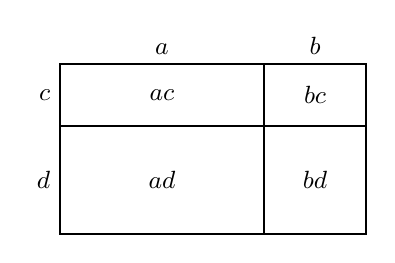
\begin{tikzpicture}[scale=0.72]
  \draw[thick] (0,0) rectangle (5.4,3.0);
  \draw[thick] (3.6,0) -- (3.6,3.0);
  \draw[thick] (0,1.9) -- (5.4,1.9);
  \node[font=\small] at (1.8,2.45) {$ac$};
  \node[font=\small] at (4.5,2.45) {$bc$};
  \node[font=\small] at (1.8,0.95) {$ad$};
  \node[font=\small] at (4.5,0.95) {$bd$};
  \node[above, font=\small] at (1.8,3.0) {$a$};
  \node[above, font=\small] at (4.5,3.0) {$b$};
  \node[left, font=\small] at (0,2.45) {$c$};
  \node[left, font=\small] at (0,0.95) {$d$};
\end{tikzpicture}

{\small A distributividade dupla em \omterm{def:g6:measure:area}{áreas}: o retângulo
$(a+b) \times (c+d)$ se reparte em quatro retângulos menores --- um por
termo do desenvolvimento.}
\end{omfigure}

\begin{method}[Desenvolver e reduzir]\label{met:g8:equations:reduce}
\begin{enumerate}
  \item Desenvolva todo \omterm{def:g2:mult:def}{produto}, escrevendo cada termo com o sinal
        dele;
  \item junte os termos semelhantes ($x^2$ com $x^2$, $x$ com $x$,
        números com números);
  \item confira com um valor: substitua, por exemplo, $x = 2$ na
        expressão original e no resultado --- resultados iguais pegam a
        maioria dos erros.
\end{enumerate}
\end{method}

\section{Resolver equações}

\begin{definition}[Equação]\label{def:g8:equations:def}
Uma \emph{equação}\index{equação} é uma igualdade com um número
desconhecido, escrito $x$ (ou qualquer letra). \emph{Resolvê-la} é
encontrar todos os valores de $x$ que tornam a igualdade verdadeira ---
as \emph{soluções}.
\end{definition}

\begin{theorem}[Regras da balança]\label{thm:g8:equations:balance}
Uma \omterm{def:g8:equations:def}{equação} mantém exatamente as mesmas soluções quando:
\begin{enumerate}
  \item o mesmo número é somado aos (ou subtraído dos) dois lados;
  \item os dois lados são multiplicados (ou divididos) pelo mesmo
        número \emph{não nulo}.
\end{enumerate}
\end{theorem}
\admitted

\begin{omfigure}
\begin{tikzpicture}[scale=0.9]
  \draw[thick] (0,0) -- (0,0.5);
  \draw[thick] (-2.6,0.5) -- (2.6,0.5);
  \draw[thick] (-0.5,0) -- (0.5,0);
  \draw[thick] (-2.2,0.5) -- (-2.2,0.75);
  \draw[thick] (2.2,0.5) -- (2.2,0.75);
  \draw[omDef, fill=omDef!15] (-2.8,0.75) rectangle (-1.6,1.45);
  \node[font=\small] at (-2.2,1.1) {$x{+}3$};
  \draw[omThm, fill=omThm!15] (1.75,0.75) rectangle (2.65,1.45);
  \node[font=\small] at (2.2,1.1) {$8$};
  \node[below, font=\small] at (0,-0.25)
    {tire $3$ dos dois pratos: $x = 5$};
\end{tikzpicture}

{\small Uma \omterm{def:g8:equations:def}{equação} é uma balança equilibrada: o que se faz num prato
tem de ser feito no outro, e o equilíbrio --- a igualdade ---
sobrevive.}
\end{omfigure}

\begin{method}[Resolver uma equação do primeiro grau]\label{met:g8:equations:solve}
\begin{enumerate}
  \item Desenvolva e reduza cada lado, se for preciso;
  \item some ou subtraia nos dois lados para juntar os termos em $x$ de
        um lado e os números puros do outro;
  \item reduza e depois divida os dois lados pelo coeficiente de $x$;
  \item \emph{confira} substituindo o valor encontrado na \omterm{def:g8:equations:def}{equação}
        original.
\end{enumerate}
\end{method}

\begin{example}\label{ex:g8:equations:solve}
Resolva $7x - 5 = 4x + 16$:
\begin{align*}
7x - 5 &= 4x + 16 \\
7x - 4x &= 16 + 5
&& \text{(some $5$ e subtraia $4x$, nos dois lados)} \\
3x &= 21 \\
x &= 7 && \text{(divida os dois lados por 3).}
\end{align*}
Conferência: lado esquerdo $7 \times 7 - 5 = 44$; lado direito
$4 \times 7 + 16 = 44$. A solução é $7$.
\end{example}

\begin{example}[Com parênteses e negativos]\label{ex:g8:equations:brackets}
Resolva $3(x - 4) = 5 - 2(x + 1)$:
\begin{align*}
3x - 12 &= 5 - 2x - 2 && \text{(desenvolva os dois lados)} \\
3x - 12 &= 3 - 2x && \text{(reduza)} \\
5x &= 15 && \text{(some $2x + 12$ nos dois lados)} \\
x &= 3 .
\end{align*}
Conferência: $3(3 - 4) = -3$ e $5 - 2(3+1) = 5 - 8 = -3$. \quad
Solução: $3$.
\end{example}

\begin{method}[Resolver um problema com uma equação]\label{met:g8:equations:problem}
\begin{enumerate}
  \item Escolha a incógnita: ``seja $x$ \dots'' (a quantidade pedida ou
        outra mais simples relacionada a ela);
  \item traduza a história numa \omterm{def:g8:equations:def}{equação};
  \item resolva-a;
  \item interprete: responda à pergunta original com uma frase, com
        unidades, e confira a resposta com a história.
\end{enumerate}
\end{method}

\begin{example}\label{ex:g8:equations:problem}
Lucas é $4$ anos mais velho que a irmã; juntas, as idades deles somam
$26$. Seja $x$ a idade da irmã; então Lucas tem $x + 4$, e
\[
x + (x + 4) = 26
\ \Longrightarrow\
2x + 4 = 26
\ \Longrightarrow\
2x = 22
\ \Longrightarrow\
x = 11 .
\]
A irmã tem $11$ anos e Lucas tem $15$. Confere: $11 + 15 = 26$ e
$15 - 11 = 4$.
\end{example}

\section{Ordem e desigualdades}

\begin{proposition}[Operações e ordem]\label{prop:g8:equations:order}
Somar o mesmo número aos dois lados de uma desigualdade a preserva;
multiplicar os dois lados por um número \emph{positivo} a preserva;
multiplicar por um número \emph{negativo} a \emph{inverte}:
\[
2 < 5 \ \text{ mas }\ (-1) \times 2 > (-1) \times 5 .
\]
\end{proposition}
\admitted

\begin{example}\label{ex:g8:equations:inequality}
Resolva $5 - 2x \leq 11$: subtraia $5$ dos dois lados, $-2x \leq 6$;
divida por $-2$ \emph{e inverta}: $x \geq -3$. Todos os números maiores
ou iguais a $-3$ são soluções --- uma \omterm{def:g8:equations:def}{equação} em geral tem uma solução,
e uma desigualdade tem uma semirreta inteira delas.
\end{example}

\section{Exercícios}

\begin{exercise}[$\star$]\label{exo:g8:equations:1}
Desenvolva e reduza:
\[
5(2x + 3), \qquad
-3(4x - 1), \qquad
2(3x - 2) + 4(x + 5).
\]
\end{exercise}

\begin{exercise}[$\star$]\label{exo:g8:equations:2}
Desenvolva e reduza:
\[
(x + 2)(x + 7), \qquad
(3x + 1)(2x - 5), \qquad
(x - 4)(x - 6).
\]
\end{exercise}

\begin{exercise}[$\star$]\label{exo:g8:equations:3}
$x = 3$ é solução de $4x - 5 = 7$? E de $2x + 1 = x + 4$? E de
$x^2 = 6x - 9$? (Substitua e compare os dois lados.)
\end{exercise}

\begin{exercise}[$\star$]\label{exo:g8:equations:4}
Resolva, com conferência:
\[
x + 9 = 4, \qquad
5x = -35, \qquad
\frac{x}{3} = 8, \qquad
2x - 7 = 13 .
\]
\end{exercise}

\begin{exercise}[$\star$]\label{exo:g8:equations:5}
Resolva:
\[
6x + 5 = 2x + 25, \qquad
9 - 4x = x - 11, \qquad
3(x + 2) = 2x + 11 .
\]
\end{exercise}

\begin{exercise}[$\star$]\label{exo:g8:equations:6}
Resolva $4(2x - 3) = 5(x + 6)$, desenvolvendo primeiro, e confira a sua
solução.
\end{exercise}

\begin{exercise}[$\star$]\label{exo:g8:equations:7}
Traduza e resolva: ``o triplo de um número, diminuído de $8$, é igual a
$19$''; ``o dobro de um número aumentado de $5$ é igual ao número
aumentado de $12$''.
\end{exercise}

\begin{exercise}[$\star\star$]\label{exo:g8:equations:8}
O comprimento de um retângulo é $5$ cm maior que a largura dele, e o
\omterm{def:g6:measure:perimeter}{perímetro} é $58$ cm. Seja $x$ a largura: escreva uma \omterm{def:g8:equations:def}{equação},
resolva-a e dê as duas dimensões.
\end{exercise}

\begin{exercise}[$\star\star$]\label{exo:g8:equations:9}
Três números inteiros consecutivos têm \omterm{def:g1:addition:def}{soma} $141$. Chame o do meio de
$n$ e encontre os três.
\end{exercise}

\begin{exercise}[$\star\star$]\label{exo:g8:equations:10}
Resolva as desigualdades e descreva as soluções:
\[
3x + 4 > 19, \qquad
7 - 2x \geq 1, \qquad
5(x - 1) < 2x + 7 .
\]
\end{exercise}

\begin{exercise}[$\star\star$]\label{exo:g8:equations:11}
Mia tem $140$ reais de poupança e acrescenta $15$ reais por mês; Tomás
tem $200$ reais e acrescenta $10$ reais por mês. Depois de quantos
meses Mia terá estritamente mais que Tomás? (Monte uma
desigualdade.)
\end{exercise}

\begin{exercise}[$\star\star\star$]\label{exo:g8:equations:12}
Resolva a \omterm{def:g8:equations:def}{equação} $\dfrac{x + 3}{4} = \dfrac{2x - 1}{5}$. (Multiplique
os dois lados por $20$, o \omterm{def:g4:fractions:def}{denominador} comum, e depois siga como de
costume; confira a sua solução na \omterm{def:g8:equations:def}{equação} original.)
\end{exercise}

\section{Problema: produtos notáveis e a escada dos números
ímpares}

\begin{problem}[{Problema de fim de semana --- $(a+b)^2$, $(a-b)^2$,
$(a+b)(a-b)$, e a soma $1 + 3 + 5 + \dots + (2n-1) = n^2$}]
\label{pb:g8:equations:1}
Três desenvolvimentos aparecem com tanta frequência que a álgebra os
sabe de cor: são os \emph{\omterm{def:g2:mult:def}{produtos} notáveis}. Este problema os deduz da
distributividade dupla (\cref{thm:g8:equations:expand}), transforma-os
num superpoder de cálculo mental, usa-os para demonstrar um fato lindo
sobre os \omterm{def:g3:numbers:evenodd}{números ímpares} e termina resolvendo \omterm{def:g8:equations:def}{equações} de um tipo
inteiramente novo: \omterm{def:g8:equations:def}{equações} com um quadrado dentro.

\medskip
\noindent\textbf{Parte I --- Os três \omterm{def:g2:mult:def}{produtos} notáveis.}
\begin{enumerate}
  \item Desenvolva $(a + b)^2 = (a + b)(a + b)$ e reduza, para
        demonstrar
        \[
        (a + b)^2 = a^2 + 2ab + b^2 .
        \]
  \item Demonstre do mesmo modo os dois companheiros:
        \[
        (a - b)^2 = a^2 - 2ab + b^2,
        \qquad
        (a + b)(a - b) = a^2 - b^2 .
        \]
  \item Trace um quadrado de lado $a + b$, divida cada lado em $a$ e
        $b$ e corte o quadrado em quatro peças. Que parte da primeira
        identidade cada pedaço do desenho representa?
  \item Cálculo mental: use os \omterm{def:g2:mult:def}{produtos} notáveis para calcular, sem
        armar nenhuma multiplicação,
        \[
        101^2, \qquad 99^2, \qquad 49 \times 51 .
        \]
  \item Uma armadilha clássica: Zoe escreve
        ``$(a + b)^2 = a^2 + b^2$''. Teste a fórmula dela com $a = 3$ e
        $b = 4$ e explique, no desenho da questão 3, exatamente que
        peças a fórmula dela esquece.
\end{enumerate}

\medskip
\noindent\textbf{Parte II --- A escada dos \omterm{def:g3:numbers:evenodd}{números ímpares}.}
\begin{enumerate}[resume]
  \item Calcule $1$, depois $1 + 3$, depois $1 + 3 + 5$, depois
        $1 + 3 + 5 + 7$, depois $1 + 3 + 5 + 7 + 9$. O que você percebe
        nos resultados?
  \item Explique por que o $n$-ésimo \omterm{def:g3:numbers:evenodd}{número ímpar} é $2n - 1$ (confira:
        $n = 1, 2, 3$ dão $1, 3, 5$).
  \item Use um \omterm{def:g2:mult:def}{produto} notável da Parte I para desenvolver e reduzir
        $(n + 1)^2 - n^2$. O que o resultado tem a ver com a questão
        7?
  \item A questão 8 diz: para passar de um quadrado de lado $n$ a um
        quadrado de lado $n + 1$, acrescenta-se exatamente o próximo
        \omterm{def:g3:numbers:evenodd}{número ímpar} de casinhas --- uma borda em forma de L ao longo
        de dois lados, mais o canto. Partindo de $1 = 1^2$ e fazendo o
        quadrado crescer uma camada de cada vez, explique por que
        \[
        1 + 3 + 5 + \dots + (2n - 1) = n^2 :
        \]
        a \omterm{def:g1:addition:def}{soma} dos $n$ primeiros \omterm{def:g3:numbers:evenodd}{números ímpares} é o $n$-ésimo
        quadrado.
  \item Deduza, sem somar um a um: o valor de
        $1 + 3 + 5 + \dots + 99$; e quantos \omterm{def:g3:numbers:evenodd}{números ímpares}, a partir
        de $1$, somam exatamente $400$.
\end{enumerate}

\medskip
\noindent\textbf{Parte III --- \omterm{def:g8:equations:def}{Equações} com um quadrado.}
\begin{enumerate}[resume]
  \item Reconheça um \omterm{def:g2:mult:def}{produto} notável em $x^2 + 6x + 9$ e resolva a
        \omterm{def:g8:equations:def}{equação} $x^2 + 6x + 9 = 0$.
  \item Explique, usando a regra de sinal e distância da
        \cref{thm:g8:negprod:rules}, por que um \omterm{def:g2:mult:def}{produto} de dois números
        pode ser \omterm{def:g1:counting:zero}{zero} \emph{apenas se} um dos dois fatores for \omterm{def:g1:counting:zero}{zero}.
        Use isso para resolver $(x - 2)(x + 5) = 0$.
  \item Resolva $x^2 = 49$ passando tudo para um lado e fatorando
        $x^2 - 49$ com o terceiro \omterm{def:g2:mult:def}{produto} notável. Quantas soluções
        essa \omterm{def:g8:equations:def}{equação} tem --- e em que isso difere de todas as \omterm{def:g8:equations:def}{equações}
        resolvidas neste capítulo até aqui?
  \item No \cref{exo:g8:equations:3} você conferiu que $x = 3$ é
        solução de $x^2 = 6x - 9$. Mostre que ela é a \emph{única}:
        passe tudo para um lado, reconheça um \omterm{def:g2:mult:def}{produto} notável e
        conclua.
  \item Final: calcule $2026^2 - 2025^2$ de cabeça e explique, com um
        \omterm{def:g2:mult:def}{produto} notável, por que a \omterm{ex:g1:subtraction:difference}{diferença} de dois quadrados
        consecutivos é sempre a \omterm{def:g1:addition:def}{soma} dos dois números --- o que é a
        questão 8 outra vez.
\end{enumerate}
\end{problem}
